%----------------------------------------------------------------------------------------------
%-----------------------------------     1 Reelle Zahlen     ----------------------------------
%----------------------------------------------------------------------------------------------

\section{Reelle Zahlen}

\begin{tabular}{ll | ll} 
    Zahlenmengen:   & S. 1, 331, 335    & Mengenlehre:      & S. 335, 1230  \\ 
    Summenzeichen:  & S. 6-7            & Produktzeichen:   & S. 7          \\
    Beweismethoden: & S. 5-6            & Fakultät          & S. 13         \\
\end{tabular}

%----------------------------------------------------------------------------------------------
%----------------------------------     1.1 Zahlenmengen     ----------------------------------
%----------------------------------------------------------------------------------------------
\subsection{Zahlenmengen}{1, 331}		
\renewcommand{\arraystretch}{1.2}
% TODO Space before and after = a bit larger
\begin{tabular}{ll @{}c@{} l} 
    Ganze Zahlen:       & $\mathbb{Z}$      & $=$   & $\left\{\ldots,-2,-1,0,1,2,\ldots \right\}; $ \\
    Natürliche Zahlen:  & $\mathbb{N}$      & $=$   & $\left\{1,2,3,\ldots\right\};$                \\
                        & $\mathbb{N}_0$    & $=$   & $\left\{0,1,2,3,\ldots\right\};$              \\
    Rationale Zahlen:   & $\mathbb{Q}$      & $=$   & $\left\{x \, | \, x \;=\; \frac{p}{q} \text{ mit } p \in \mathbb{Z} \text{ und } (q \in \mathbb{Z} \smallsetminus \{0\})\right\};$ \\
    Irrationale Zahlen: &                   &       & nichtperiodische Kommazahlen \\
    Reelle Zahlen:      & $\mathbb{R}$      & $=$   & z.B. $\sqrt{2}, \pi,\phi$\\
    Komplexe Zahlen     & $\mathbb{C}$      & $=$   & $\left\{a + bi \,| \, a, b \epsilon \mathbb{R} \right\}$
\end{tabular}

%----------------------------------------------------------------------------------------------
%------------------------------     1.2 Supremum und Infimum     ------------------------------
%----------------------------------------------------------------------------------------------
\subsection{Supremum und Infimum \hspace{0.3cm}\texorpdfstring{$\Rightarrow$}{→} \hspace{0.3cm}3. Folgen}
\begin{tabular}{ll} 
    $\sup(X)$   & Kleinste obere Schranke \textrightarrow\ {\color{red}M}aximum ist immer auch Supremum \\
    $\inf(X)$   & Grösste untere Schranke \textrightarrow\ {\color{red}m}inimum ist immer auch Infimum
\end{tabular}
\renewcommand{\arraystretch}{1} \\ \\

\hspace{0.3cm}
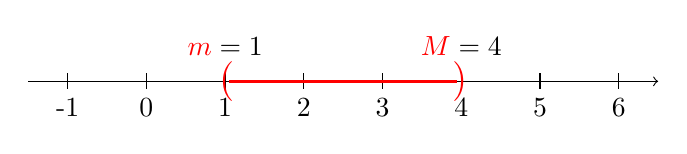
\begin{tikzpicture}[x=1cm]
    % Zahlenstrahl
    \draw[->] (-1.5,0) -- (6.5,0);

    % Ticks und Zahlen
    \foreach \x in {-1,0,1,2,3,4,5,6} {
        \draw (\x,0.1) -- (\x,-0.1);
        \node[below] at (\x,-0.1) {\x};
    }

    % Dicke rote Linie (Menge)
    \draw[red, very thick] (1.05,0) -- (3.95,0);

    % Klammern für Infimum und Supremum
    \node[red] at (1.02,0) {\Large(};
    \node[red] at (3.98,0) {\Large)};

    % Beschriftung
    \node[above] at (1,0.2) {${\color{red}m} = 1$};
    \node[above] at (4,0.2) {${\color{red}M} = 4$};
\end{tikzpicture}\\

\begin{tabular}{ll} 
    Maximum: $\max A \in A$, größtes Element der Menge.\\
    Supremum: $\sup A$, kleinste obere Schranke, muss nicht in $A$ liegen.\\
    \textbf{Merksatz:} Maximum ${\textcolor{darkgreen}{\Rightarrow}}$ Supremum, aber Supremum ${\textcolor{red}{\not\Rightarrow}}$ Maximum.\\
    Minimum: $\min A \in A$, kleinstes Element der Menge.\\
    Infimum: $\inf A$, größte untere Schranke, muss nicht in $A$ liegen.\\
    \textbf{Merksatz:} Minimum ${\textcolor{darkgreen}{\Rightarrow}}$ Infimum, aber Infimum ${\textcolor{red}{\not\Rightarrow}}$ Minimum.
\end{tabular}
\renewcommand{\arraystretch}{1} 
\\

%----------------------------------------------------------------------------------------------
%------------------------------------     1.3 Umgebung     ------------------------------------
%----------------------------------------------------------------------------------------------
\subsection{Umgebung}
\renewcommand{\arraystretch}{1.2}
\begin{tabular}{ll} 
    Jedes offene Intervall, dass die Zahl $x_0$ enth"alt, \\ 
    heisst eine Umgebung von $x_0$ &  $U(x_0)$\\
    \\
    Es sei $\varepsilon > 0$. Unter der $\varepsilon$-Umgebung von $x_0$ \\
    versteht man das offene Intervall $(x_0-\varepsilon,x_0+\varepsilon)$ & $U_\varepsilon(x_0)$ 
\end{tabular}\\

\hspace{0.5cm}
\renewcommand{\arraystretch}{0.4}
\begin{tabular}{ll} 
    {\large $\varepsilon$}-Umgebung: & $U_\varepsilon(3)$  $=$ 
    $\{x\in\mathbb{R}\mid |x-x_0|<\varepsilon\}=(x_0-\varepsilon,\;x_0+\varepsilon)$
\end{tabular}

\hspace{0.52cm}
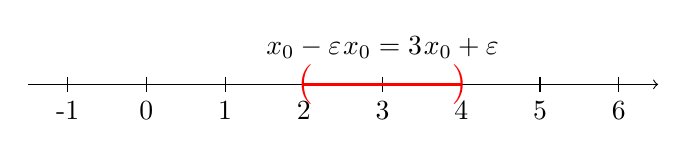
\begin{tikzpicture}[x=1cm]
    % Zahlenstrahl
    \draw[->] (-1.5,0) -- (6.5,0);

    % Ticks und Zahlen
    \foreach \x in {-1,0,1,2,3,4,5,6} {
        \draw (\x,0.1) -- (\x,-0.1);
        \node[below] at (\x,-0.1) {\x};
    }

    % Dicke rote Linie für Umgebung
    \def\xzero{3}        % x0
    \def\eps{1}          % ε
    \draw[red, very thick] (\xzero-\eps,0) -- (\xzero+\eps,0);

    % Klammern für die Umgebung
    \node[red] at ({\xzero-\eps+0.02},0) {\Large(};
    \node[red] at ({\xzero+\eps-0.025},0) {\Large)};

    % Beschriftung
    \node[above] at (\xzero,0.2) {$x_0 = \xzero$};
    \node[above] at ({\xzero-\eps},0.2) {$x_0-\varepsilon$};
    \node[above] at ({\xzero+\eps},0.2) {$x_0+\varepsilon$};
\end{tikzpicture}\\

\renewcommand{\arraystretch}{1.2}
\begin{tabular}{ll} 
        Eine $\varepsilon$-Umgebung von $x_0$ ohne die Zahl $x_0$ selbst \\
    wird punktierte $\varepsilon$-Umgebung von $x_0$ genannt & $\dot{U}_\varepsilon(x_0)=U_\varepsilon(x_0)\smallsetminus{x_0}$
\end{tabular}\\

\hspace{1.35cm}
\begin{tabular}{ll} 
    {\large $\varepsilon$}-$\dot{\text{U}}$mgebung: & $\dot{U}_\varepsilon(3)$ $=$ 
    $\{x \in \mathbb{R} \mid |x - x_0| < \varepsilon\} \setminus \{3\}$\\
\end{tabular}

\hspace{0.52cm}
\begin{tikzpicture}[x=1cm]
    % Zahlenstrahl
    \draw[->] (-1.5,0) -- (6.5,0);

    % Ticks und Zahlen
    \foreach \x in {-1,0,1,2,3,4,5,6} {
        \draw (\x,0.1) -- (\x,-0.1);
        \node[below] at (\x,-0.1) {\x};
    }

    % Dicke rote Linie für Umgebung
    \def\xzero{3}        % x0
    \def\eps{1}          % ε
    \draw[darkgreen, very thick] (\xzero-\eps,0) -- (\xzero,0);
    \draw[red, very thick] (\xzero+\eps,0) -- (\xzero,0);

    % Klammern für die Umgebung
    \node[darkgreen] at ({\xzero-\eps+0.02},0) {\Large(};
    \node[red] at ({\xzero+\eps-0.025},0) {\Large)};
    \node[red] at ({\xzero+0.04},0) {\Large(};
    \node[darkgreen] at ({\xzero-0.04},0) {\Large)};

    % Beschriftung
    \node[above] at (\xzero,0.2) {$x_0 = \xzero$};
    \node[above] at ({\xzero-\eps},0.2) {$x_0-\varepsilon$};
    \node[above] at ({\xzero+\eps},0.2) {$x_0+\varepsilon$};
\end{tikzpicture}

%----------------------------------------------------------------------------------------------
%---------------------------------     1.4 Endliche Reihen     --------------------------------
%----------------------------------------------------------------------------------------------
\subsection{Endliche Reihen}{19, 20}

\begin{tabular}{ll c|c ll} 
    Arithmetisch:   & $\sum\limits _{i=1}^n i = \frac{n(n+1)}{2}$ 
    & &
    Geometrisch:    & $\sum\limits _{i=0}^n q^i = \frac{q^{n+1} - 1}{q - 1}$ 
\end{tabular}

%----------------------------------------------------------------------------------------------
%-----------------------------------     1.5 Mittelwerte     ----------------------------------
%----------------------------------------------------------------------------------------------
\subsection{Mittelwerte}{20}

\renewcommand{\arraystretch}{0.3}
{\setlength{\tabcolsep}{6pt}
\begin{tabular}{ll} 
    Harmonisches Mittel (HM):    & $\displaystyle \frac{1}{n}\sum_{i=1}^n x_i = \frac{x_1 + x_2 + \cdots + x_n}{n}$ \\ \\
    Geometrisches Mittel (GM):   & $\displaystyle \left[\prod_{i=1}^n x_i\right]^{\frac{1}{n}}= \sqrt[n]{x_1 \cdot x_2 \cdots x_n}$ \\ \\
    Arithmetisches Mittel (AM):  & $\displaystyle\left[\frac{1}{n}\sum_{i=1}^n \frac{1}{x_i}\right]^{-1}=\left[\frac{1}{n}\left(\frac{1}{x_1}+\frac{1}{x_2}+\cdots+\frac{1}{x_n}\right)\right]^{-1}$ \\ \\
\end{tabular}}\\

\renewcommand{\arraystretch}{0.2} % Zeilenhöhe anpassen
\begin{center}
\begin{tabular}{c}
    \\
    $\text{HM} \,\,\, \leq \,\,\, \text{GM} \,\,\, \leq \,\,\,\text{AM}$\\\\
\end{tabular}
\end{center}

%----------------------------------------------------------------------------------------------
%------------------------------     1.6 Speziele Ungleichungen     ----------------------------
%----------------------------------------------------------------------------------------------
\subsection{Speziele Ungleichungen}{31 - 34}

\renewcommand{\arraystretch}{1}
\begin{tabular}{ll} 
    Bernoullische-Ungleichung:  &   $(1 + a)^n \geq 1 + n \cdot a$ \\
                                &   $\left\{ a \in \mathbb{R},\, a \geq -1 \land n \in \mathbb{N},\, n \geq 1 \right\}$ \\
    \\
    Binomische-Ungleichung:     &   $|a \cdot b| \leq \frac{1}{2} \cdot (a^2+b^2) \quad \text{für } a,b \in \mathbb{R}$                             
\end{tabular}

%----------------------------------------------------------------------------------------------
%------------------------------     1.7 Binomischer Satz     ----------------------------
%----------------------------------------------------------------------------------------------
\subsection{Binomischer Satz}{12}

Der Binomische Satz kann verwendet werden, um das Pascal-Dreieck zu berechnen.
$$ \text{Binomischer Satz: \quad} \left( a+b \right) ^n = \sum\limits _{k=0}^n \binom{n}{k} \cdot a^{n-k}\cdot b^k $$ 

\renewcommand{\arraystretch}{1.8}
\begin{center}
\begin{tabular}{c} 
    $\binom{n}{k}=\binom{n}{n-k}=\frac{n!}{k!\left(n-k\right)!} \quad \text{für } n \in \mathbb{N}, \; 0 \leq k \leq n$      		
\end{tabular}\\
\begin{tabular}{lr}
    $\binom{n+1}{k}=\frac{n+1}{n-k+1} \cdot \binom{n}{k}$   &   $\binom{n}{k+1}=\frac{n-k}{k+1} \cdot \binom{n}{k}$ 
\end{tabular}\\
\begin{tabular}{c}
    $\binom{n+1}{k+1}=\binom{n}{k+1} \cdot \binom{n}{k} = \binom{n}{k}+\binom{n-1}{k}+\binom{n-2}{k}+ \cdots +\binom{k}{k}$
\end{tabular}
\end{center}


%----------------------------------------------------------------------------------------------
%-----------------------------     1.7 Vollständige Induktion     -----------------------------
%----------------------------------------------------------------------------------------------
\subsection{Vollständige Induktion}{5 - 6}

\renewcommand{\arraystretch}{1}
\underline{\textbf{Beispiel: Vollständige Induktion}}
\[
\sum_{i=1}^n i = \frac{n \cdot (n+1)}{2}, \quad n \in \mathbb{N}
\]
\renewcommand{\arraystretch}{1.3}
\begin{tabular}{lll}
    (VA) für $n = 1$    &   $\displaystyle \sum_{i=1}^n i =\sum_{i=1}^1 1 = 1$    &   $\displaystyle \frac{n \cdot (n+1)}{2} = \frac{1 \cdot (1+1)}{2} = 1$ 
\end{tabular}\\
\\
\renewcommand{\arraystretch}{0.7}
\begin{tabular}{ll}
    (VE) (1)$\hspace{0.67cm}$    &  $\displaystyle \sum_{i=1}^n i \overset{\textcolor{green}{\checkmark}}{=}\frac{n \cdot (n+1)}{2}, \quad (n \in \mathbb{N})$ \\
    (VE) (2)                     &  $\displaystyle \sum_{i=1}^{n+1} i\overset{\textcolor{red}{?}}{=}\frac{(n+1) \cdot ((n+1)+1)}{2} = \frac{(n+1) \cdot (n+2)}{2}, \quad (n \in \mathbb{N})$ \\
    (VE) (3)                     &  $\displaystyle \sum_{i=1}^{n+1} i = \displaystyle \sum_{i=1}^{n} i +  \sum_{i=n+1}^{n+1} i = \frac{n \cdot (n+1)}{2} + (n + 1) = \; . . .$ \\\\
                                 &  $. . . = \frac{n \cdot (n+1)}{2} + (n + 1) =  \frac{n \cdot (n+1) + 2 \cdot(n + 1)}{2} = \frac{n^2 + n + 2n + 2}{2} = . . .$ \\\\
                                 &  $. . . = \displaystyle\frac{n^2 + n + 2n + 2}{2} =  \frac{n^2 + 3n + 2}{2} \overset{\textcolor{green}{\checkmark}}{=} \frac{(n+1)\cdot(n+2)}{2}$
\end{tabular}  

%----------------------------------------------------------------------------------------------
%----------------------------     Weiter Sachen Hier hinzufügen    ----------------------------
%----------------------------------------------------------------------------------------------